\documentclass[12pt,a4paper,article,english,firamath]{nsi}
\pagestyle{empty}
\begin{document}
\titre{The Lunes of Alhazen}
\classe{Euro 1\ere}
\maketitle
\begin{center}
    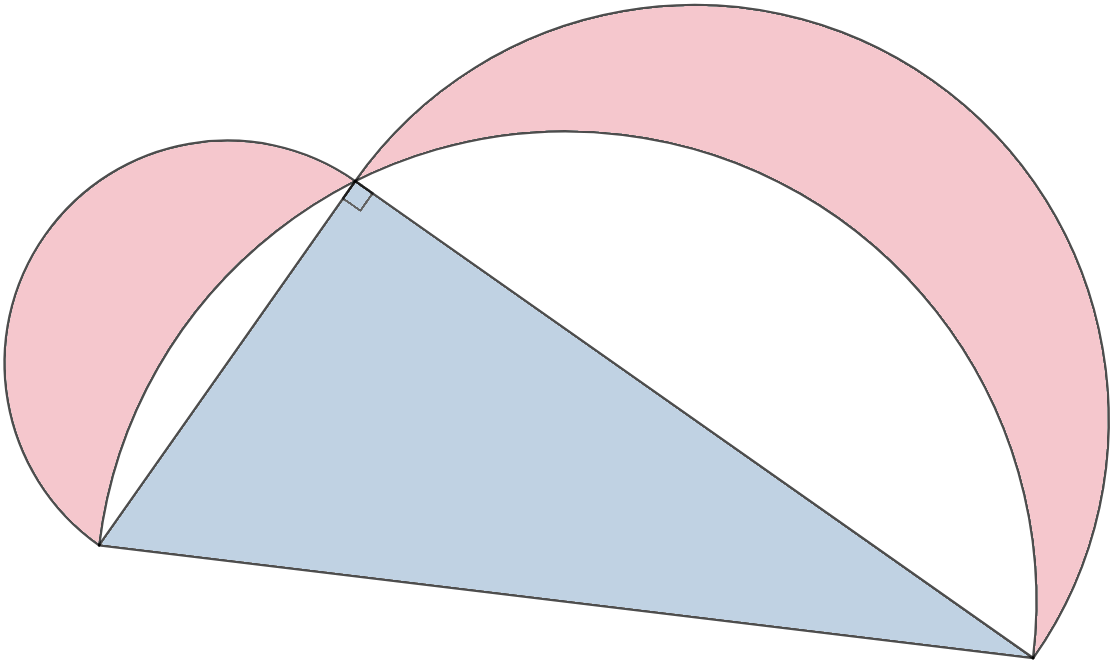
\includegraphics[width=8.5cm]{img/lunes.png}
\end{center}
The blue triangle is rectangle.\\
Can you show its area is the same as the sum of the areas of the two red lunes ?\\[13em]

\maketitle
\begin{center}
    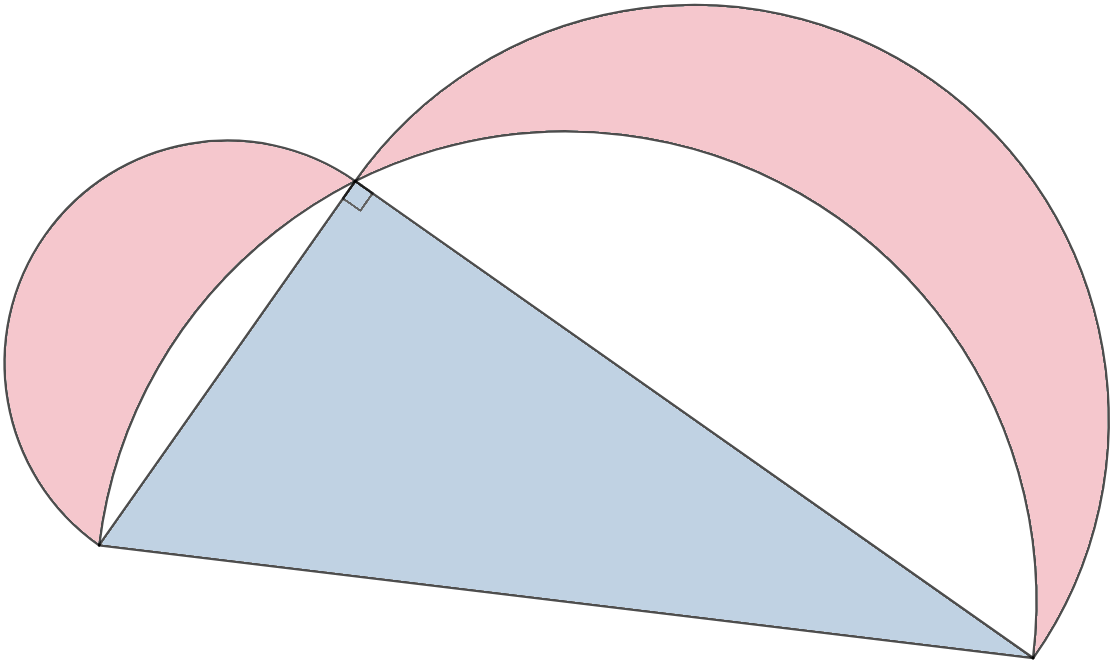
\includegraphics[width=8.5cm]{img/lunes.png}
\end{center}
The blue triangle is rectangle.\\
Can you show its area is the same as the sum of the areas of the two red lunes ?
\end{document}